\documentclass{article}
\usepackage{graphicx}
\title{Boundary Layer Adaptation}
\author{Dan Ibanez}
\date{May 17, 2014}
\begin{document}
\maketitle

This document starts to pull together the adaptive
capabilities we would like to have for boundary
layers.

\section{Thickness Adjustment}

The thickness of boundary layer $i$ is defined as:

\[t_i = t_0\cdot (r)^i\]

Where the parameters $t_0$ and $r$ are the initial
thickness and thickness ratio, respectively.
By the formula for the sum of a geometric series,
the total thickness of $n$ boundary layers is:

\[t_0\frac{1-r^n}{1-r}\]

Thickness adjustment varies these two parameters without
changing the mesh topology, including the number of boundary
layers.

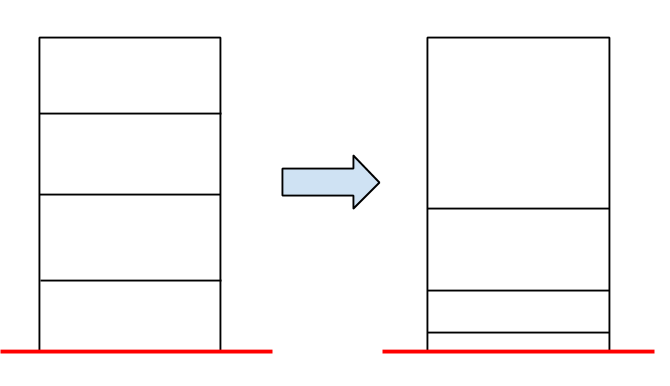
\includegraphics[width=0.6\textwidth]{thick_adapt.png}

In the special case where we restrict
\[t_0 = \frac{1-r}{1-r^n}\]
then the total thickness does not change.
If it does, however, we need a way to adapt the adjacent
unstructured mesh to account for this change.

\section{Changing Layer Count}

Another operation involves changing the number of layers $n$
without changing the thickness parameters $t_0$ and $r$.
This is easiest to consider on a simple boundary layer surface:

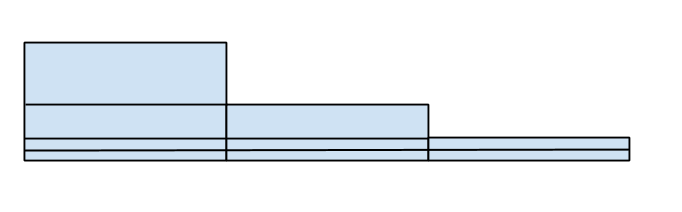
\includegraphics[width=0.6\textwidth]{layer_step.png}

There was also mention of the restriction of the ``step"
to be of height 1, i.e. adjacent stacks can only differ in
height by $\pm 1$.
We are considering being able to lift this restriction.

Adding prisms has to (again) consider adapting the unstructured mesh,
but also introduces new complexity in the need for pyramids to
cover the newly exposed quad faces.

\section{Deforming Geometry}

There are problems in which the geometric model itself deforms in various
ways (flexible aerodynamic surface, etc.).
This is closely related to the issues above of adapting the unstructured
mesh due to a change in the position of the boundary layer.
It should actually be considered as a problem independent of boundary layers,
such as snapping.

\section{Model Edges}

When two boundary layered model surfaces come together at an edge,
the boundary layers have to be somehow reconciled.
Here are a couple examples which illustrate how this may be a concern
for MeshAdapt:

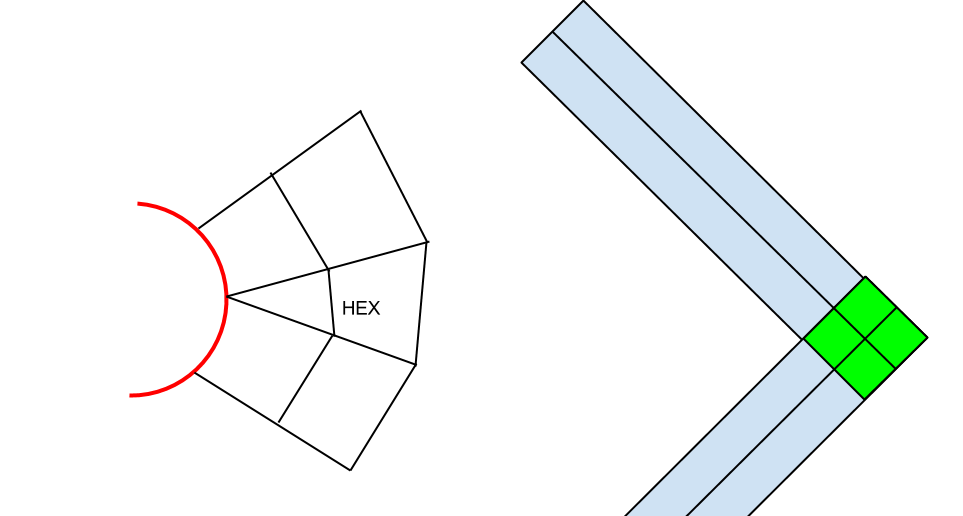
\includegraphics[width=0.6\textwidth]{layer_blend.png}

\section{Mesh Generation}

Our meshes almost always come from the Simmetrix generator, so when
we strictly define a boundary layer, including all the literal
corner cases, we need to make sure that definition is consistent
with the meshes Simmetrix generates.

As a prerequisite to that, we need to gather a list of all the configuration
options for Simmetrix mesh generation and how they affect the structure
of the mesh with respect to boundary layers.

\end{document}
